% Figures/hemicontinuity.tex
% Illustrates Example \ref{eg:hemicontinuity-independent} of Chapter
% \ref{ch:maximum}: the correspondences varphi, psi, gamma on [0,1] showing that
% upper and lower hemicontinuity are logically independent.
% Source: Fukuda (2026), Supplementary Ch. 13, Example 13.4 (p. 470).
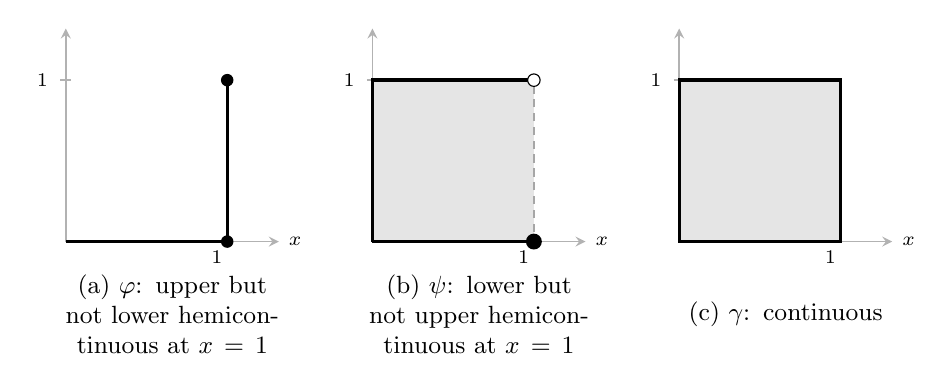
\begin{tikzpicture}[
		scale=2.05,
		>=stealth,
		axisline/.style={->,gray!60,semithick},
		graphline/.style={line width=1.2pt,black},
		excluded/.style={line width=0.7pt,gray!70,densely dashed},
		caption/.style={font=\small,text width=3.15cm,align=center},
	]

	% ---------- phi: uhc but not lhc ----------
	\begin{scope}
		\draw[axisline] (0,0) -- (1.32,0) node[right,black,font=\scriptsize] {$x$};
		\draw[axisline] (0,0) -- (0,1.32);
		\draw[gray!60,semithick] (-0.035,1) -- (0.035,1);
		\draw[gray!60,semithick] (1,-0.035) -- (1,0.035);
		\node[left,font=\scriptsize] at (-0.05,1) {$1$};
		\node[below left,font=\scriptsize,inner sep=1.5pt] at (1,-0.03) {$1$};
		\draw[graphline] (0,0) -- (1,0);
		\draw[graphline] (1,0) -- (1,1);
		\fill (1,1) circle (1.1pt);
		\fill (1,0) circle (1.1pt);
		\node[caption] at (0.66,-0.45) {(a)~$\varphi$: upper but not lower
			hemicontinuous at $x=1$};
	\end{scope}

	% ---------- psi: lhc but not uhc ----------
	\begin{scope}[shift={(1.9,0)}]
		\fill[black!10] (0,0) rectangle (1,1);
		\draw[axisline] (0,0) -- (1.32,0) node[right,black,font=\scriptsize] {$x$};
		\draw[axisline] (0,0) -- (0,1.32);
		\draw[gray!60,semithick] (-0.035,1) -- (0.035,1);
		\node[left,font=\scriptsize] at (-0.05,1) {$1$};
		\node[below left,font=\scriptsize,inner sep=1.5pt] at (1,-0.03) {$1$};
		\draw[graphline] (0,0) -- (0,1) -- (1,1);
		\draw[graphline] (0,0) -- (1,0);
		\draw[excluded] (1,0.06) -- (1,1);
		\draw[fill=white] (1,1) circle (1.1pt);
		\fill (1,0) circle (1.4pt);
		\node[caption] at (0.66,-0.45) {(b)~$\psi$: lower but not upper
			hemicontinuous at $x=1$};
	\end{scope}

	% ---------- gamma: continuous ----------
	\begin{scope}[shift={(3.8,0)}]
		\fill[black!10] (0,0) rectangle (1,1);
		\draw[axisline] (0,0) -- (1.32,0) node[right,black,font=\scriptsize] {$x$};
		\draw[axisline] (0,0) -- (0,1.32);
		\draw[gray!60,semithick] (-0.035,1) -- (0.035,1);
		\node[left,font=\scriptsize] at (-0.05,1) {$1$};
		\node[below left,font=\scriptsize,inner sep=1.5pt] at (1,-0.03) {$1$};
		\draw[graphline] (0,0) rectangle (1,1);
		\node[caption] at (0.66,-0.45) {(c)~$\gamma$: continuous};
	\end{scope}

\end{tikzpicture}
